% Created 2021-04-20 Tue 19:43
% Intended LaTeX compiler: pdflatex

\documentclass[english]{article}
\usepackage[T1, T2A]{fontenc}
\usepackage[lutf8]{luainputenc}
\usepackage[english, russian]{babel}
\usepackage{minted}
\usepackage{graphicx}
\usepackage{longtable}
\usepackage{hyperref}
\usepackage{xcolor}
\usepackage{natbib}
\usepackage{amssymb}
\usepackage{stmaryrd}
\usepackage{amsmath}
\usepackage{caption}
\usepackage{mathtools}
\usepackage{amsthm}
\usepackage{tikz}
\usepackage{grffile}
\usepackage{extarrows}
\usepackage{wrapfig}
\usepackage{algorithm}
\usepackage{algorithmic}
\usepackage{lipsum}
\usepackage{rotating}
\usepackage{placeins}
\usepackage[normalem]{ulem}
\usepackage{amsmath}
\usepackage{textcomp}
\usepackage{capt-of}

\usepackage{geometry}
\geometry{a4paper,left=2.5cm,top=2cm,right=2.5cm,bottom=2cm,marginparsep=7pt, marginparwidth=.6in}
 \usepackage{hyperref}
 \hypersetup{
     colorlinks=true,
     linkcolor=blue,
     filecolor=orange,
     citecolor=black,      
     urlcolor=cyan,
     }

\usetikzlibrary{decorations.markings}
\usetikzlibrary{cd}
\usetikzlibrary{patterns}
\usetikzlibrary{automata, arrows}

\newcommand\addtag{\refstepcounter{equation}\tag{\theequation}}
\newcommand{\eqrefoffset}[1]{\addtocounter{equation}{-#1}(\arabic{equation}\addtocounter{equation}{#1})}
\newcommand{\llb}{\llbracket}
\newcommand{\rrb}{\rrbracket}


\newcommand{\R}{\mathbb{R}}
\renewcommand{\C}{\mathbb{C}}
\newcommand{\N}{\mathbb{N}}
\newcommand{\A}{\mathfrak{A}}
\newcommand{\B}{\mathfrak{B}}
\newcommand{\rank}{\mathop{\rm rank}\nolimits}
\newcommand{\const}{\var{const}}
\newcommand{\grad}{\mathop{\rm grad}\nolimits}

\newcommand{\todo}{{\color{red}\fbox{\text{Доделать}}}}
\newcommand{\fixme}{{\color{red}\fbox{\text{Исправить}}}}

\newcounter{propertycnt}
\setcounter{propertycnt}{1}
\newcommand{\beginproperty}{\setcounter{propertycnt}{1}}

\theoremstyle{plain}
\newtheorem{propertyinner}{Свойство}
\newenvironment{property}{
  \renewcommand\thepropertyinner{\arabic{propertycnt}}
  \propertyinner
}{\endpropertyinner\stepcounter{propertycnt}}
\newtheorem{axiom}{Аксиома}
\newtheorem{lemma}{Лемма}
\newtheorem{manuallemmainner}{Лемма}
\newenvironment{manuallemma}[1]{%
  \renewcommand\themanuallemmainner{#1}%
  \manuallemmainner
}{\endmanuallemmainner}

\theoremstyle{remark}
\newtheorem*{remark}{Примечание}
\newtheorem*{solution}{Решение}
\newtheorem{corollary}{Следствие}[theorem]
\newtheorem*{examp}{Пример}
\newtheorem*{observation}{Наблюдение}

\theoremstyle{definition}
\newtheorem{task}{Задача}
\newtheorem{theorem}{Теорема}[section]
\newtheorem*{definition}{Определение}
\newtheorem*{symb}{Обозначение}
\newtheorem{manualtheoreminner}{Теорема}
\newenvironment{manualtheorem}[1]{%
  \renewcommand\themanualtheoreminner{#1}%
  \manualtheoreminner
}{\endmanualtheoreminner}
\captionsetup{justification=centering,margin=2cm}
\newenvironment{colored}[1]{\color{#1}}{}

\tikzset{->-/.style={decoration={
  markings,
  mark=at position .5 with {\arrow{>}}},postaction={decorate}}}
\makeatletter
\newcommand*{\relrelbarsep}{.386ex}
\newcommand*{\relrelbar}{%
  \mathrel{%
    \mathpalette\@relrelbar\relrelbarsep
  }%
}
\newcommand*{\@relrelbar}[2]{%
  \raise#2\hbox to 0pt{$\m@th#1\relbar$\hss}%
  \lower#2\hbox{$\m@th#1\relbar$}%
}
\providecommand*{\rightrightarrowsfill@}{%
  \arrowfill@\relrelbar\relrelbar\rightrightarrows
}
\providecommand*{\leftleftarrowsfill@}{%
  \arrowfill@\leftleftarrows\relrelbar\relrelbar
}
\providecommand*{\xrightrightarrows}[2][]{%
  \ext@arrow 0359\rightrightarrowsfill@{#1}{#2}%
}
\providecommand*{\xleftleftarrows}[2][]{%
  \ext@arrow 3095\leftleftarrowsfill@{#1}{#2}%
}
\makeatother

\newenvironment{rualgo}[1][]
  {\begin{algorithm}[#1]
     \selectlanguage{russian}%
     \floatname{algorithm}{Алгоритм}%
     \renewcommand{\algorithmicif}{{\color{red}\textbf{если}}}%
     \renewcommand{\algorithmicthen}{{\color{red}\textbf{тогда}}}%
     \renewcommand{\algorithmicelse}{{\color{red}\textbf{иначе}}}%
     \renewcommand{\algorithmicend}{{\color{red}\textbf{конец}}}%
     \renewcommand{\algorithmicfor}{{\color{red}\textbf{для}}}%
     \renewcommand{\algorithmicto}{{\color{red}\textbf{до}}}%
     \renewcommand{\algorithmicdo}{{\color{red}\textbf{делать}}}%
     \renewcommand{\algorithmicwhile}{{\color{red}\textbf{пока}}}%
     \renewcommand{\algorithmicrepeat}{{\color{red}\textbf{повторять}}}%
     \renewcommand{\algorithmicuntil}{{\color{red}\textbf{до тех пор пока}}}%
     \renewcommand{\algorithmicloop}{{\color{red}\textbf{повторять}}}%
     \renewcommand{\algorithmicnot}{{\color{blue}\textbf{не}}}%
     \renewcommand{\algorithmicand}{{\color{blue}\textbf{и}}}%
     \renewcommand{\algorithmicor}{{\color{blue}\textbf{или}}}%
     \renewcommand{\algorithmicrequire}{{\color{blue}\textbf{Ввод}}}%
     \renewcommand{\algorithmicensure}{{\color{blue}\textbf{Вывод}}}%
     \renewcommand{\algorithmicreturn}{{\color{red}\textbf{Вернуть}}}%
     \renewcommand{\algorithmicrtrue}{{\color{blue}\textbf{истинна}}}%
     \renewcommand{\algorithmicrfalse}{{\color{blue}\textbf{ложь}}}%
     % Set other language requirements
  }
  {\end{algorithm}}
\date{}
\title{}
\hypersetup{
 pdfauthor={},
 pdftitle={},
 pdfkeywords={},
 pdfsubject={},
 pdfcreator={Emacs 28.0.50 (Org mode 9.4.4)}, 
 pdflang={English}}
\begin{document}

\begin{titlepage}
\begin{center}
\large\textbf{Федеральное государственное автономное образовательное учреждение высшего образования ``Национальный исследовательский университет ИТМО``} \\

\vspace{0.5cm}

Факультет информационных технологий и программирования \\

\vspace{0.5cm}

Направление ``Прикладная математика и информатика`` \\



\vspace{3cm}



Отчет к лабораторной работе №2 \\

\vspace{0.5cm}

\textbf{Методы многомерной оптимизации}
\end{center}




\vfill

\begin{flushright}
\large
Выполнили студенты группы М3237 \\

\vspace{0.5cm}

Ярошевский Илья \\
Аникина Вероника \\
Крюков Александр
\end{flushright}


\vspace{3cm}

\begin{center}
Санкт-Петербург 2021
\end{center}
\end{titlepage}



\section{Цели работы}
\label{sec:org48598f1}
\begin{enumerate}
\item Реализовать алгоритмы
\begin{itemize}
\item Метод градиентного спуска
\item Метод наискорейшего спуска
\item Метод сопряженных градиентов
\end{itemize}
\item Проанализировать траектории методов для некоторых квадратичных функций
\item Исследовать количество итераций в зависимости от размерности пространства и числа обусловленности
\end{enumerate}
\section{Ход работы}
\label{sec:orgbd88cf3}
Во всех тестах начальное приближение --- вектор размерности
пространства из единиц, точность \(\varepsilon\) = 0.001, ограничение на
количество итераций --- 10000
\subsection{Количество итераций}
\label{sec:org56fe122}
\subsubsection{Метод градиентного спуска}
\label{sec:org703e44c}
\begin{center}
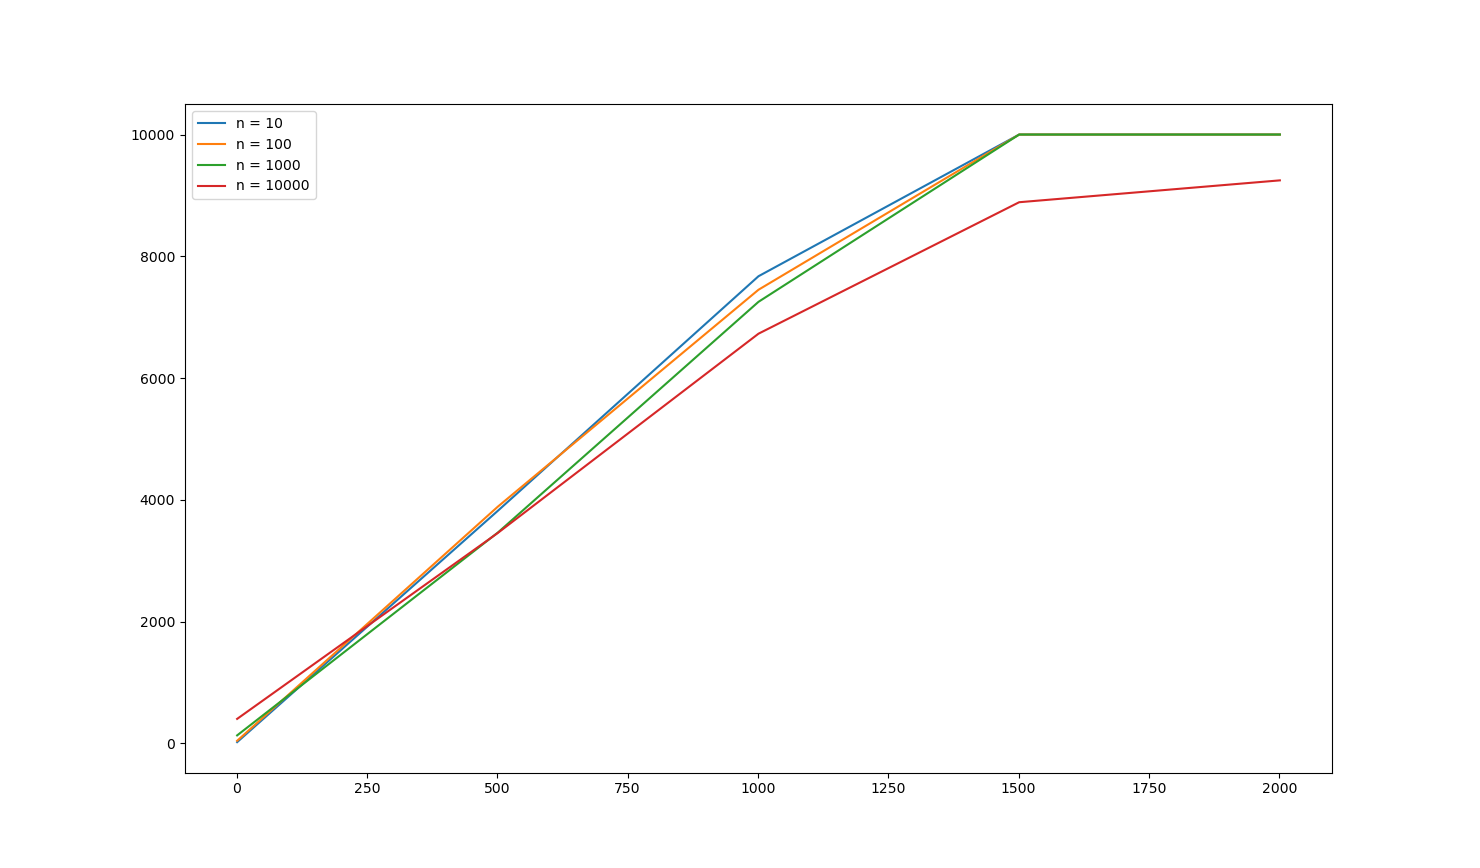
\includegraphics[scale=0.4]{plots/gradient_descent_1.png}
\end{center} Видно, что количество итераций не
зависит от размерности пространства \(n\), но линейно зависит от числа
обусловленности \(k\)
\subsubsection{Метод наискорейшего спуска}
\label{sec:org6a82da9}
\begin{center}
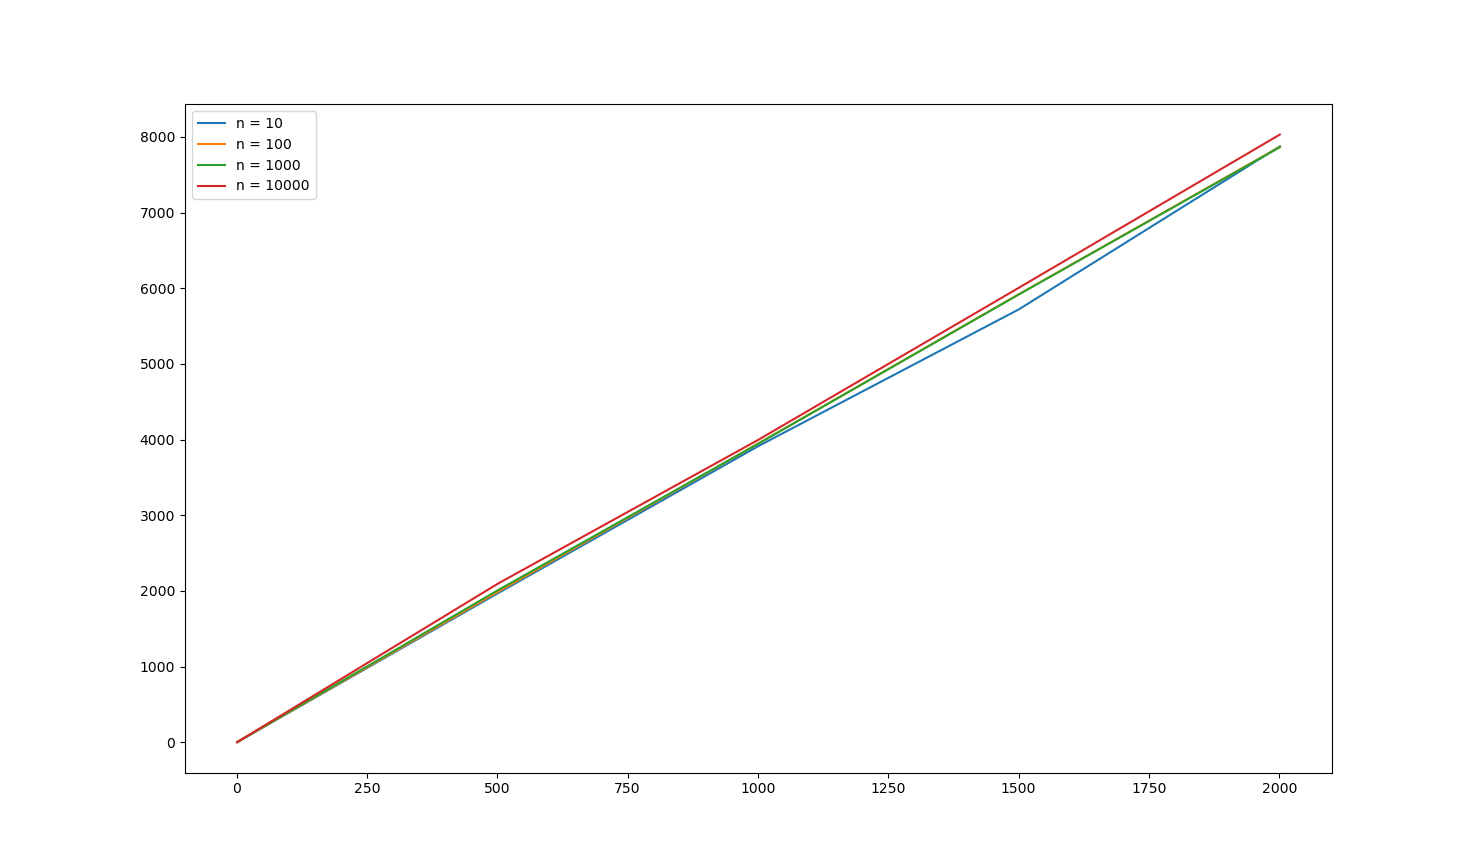
\includegraphics[scale=0.4]{plots/steepest_gradient_1.png}
\end{center} Так же как и в методе градиентного
спуска можно видеть линейную зависимость количества итераций от числа
обусловленности. Количество итераций так же не зависит от размерности
пространства.
\subsubsection{Метод сопряженный градиентов}
\label{sec:org947248c}
\begin{center}
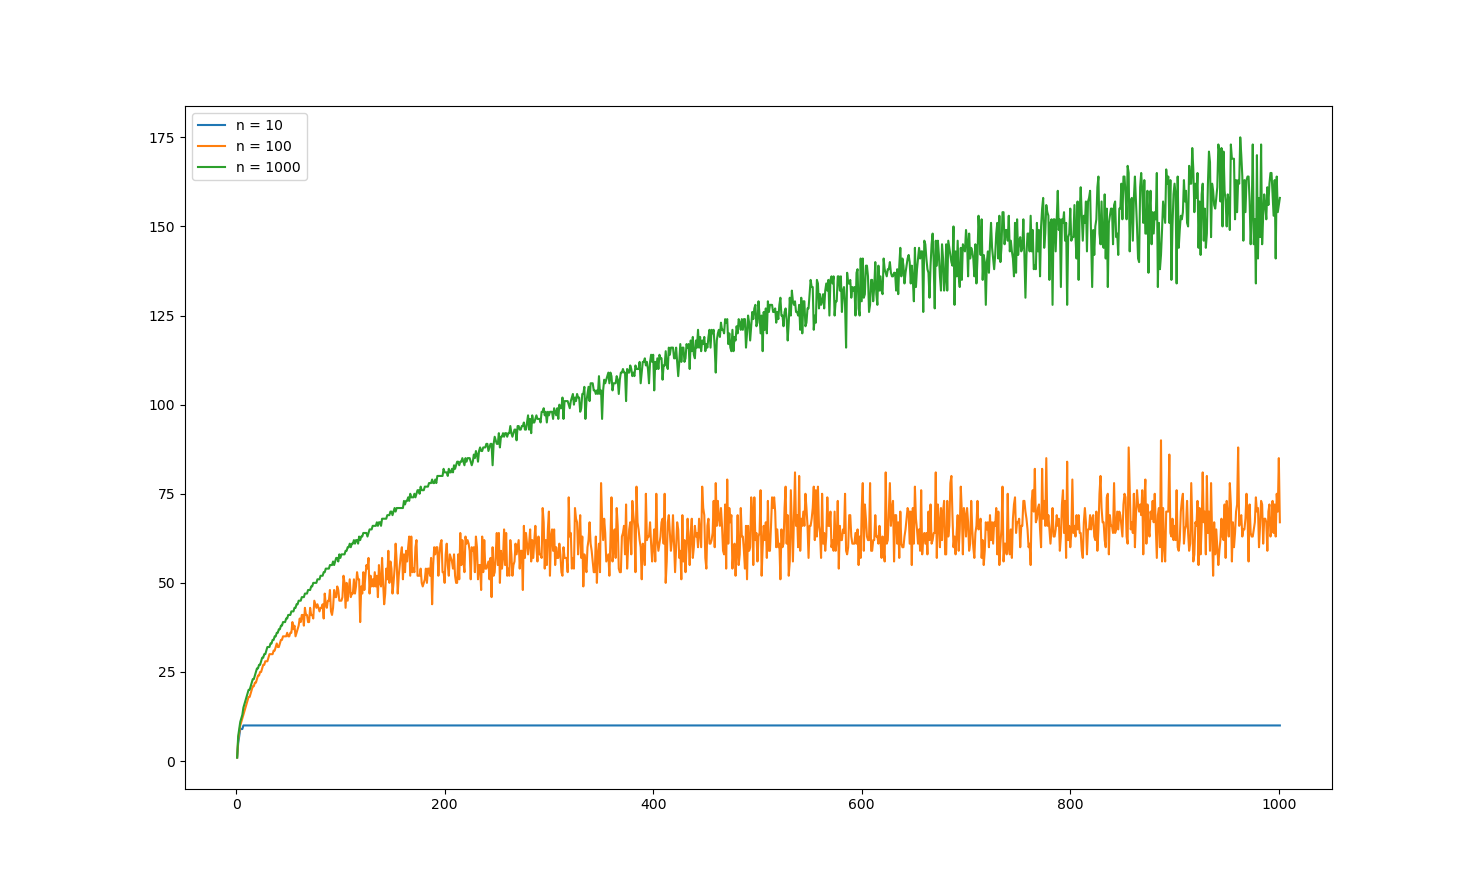
\includegraphics[scale=0.4]{plots/conjugate_gradient_1.png}
\end{center} По очевидным причинам количество
итераций для произвольной функции будет константным и равным
размерности пространства.
\subsection{Траектории}
\label{sec:org821faae}
\[ f_1(x) = \frac{1}{2}\begin{pmatrix}
100 & -1 \\
-1 & 1
\end{pmatrix} x^2 + \begin{pmatrix} -10 & 0 \end{pmatrix}x\]
Все методы находят минимум функции \(f_1^* = -0.50505\) в точке \(x^* = (0.101011\ 0.1011)\)
\[ f_2(x) = \frac{1}{2}\begin{pmatrix}
3 & -1 \\
-1 & 2
\end{pmatrix} x^2 + \begin{pmatrix} -5 & 2 \end{pmatrix}x\]
Все методы находят минимум функции \(f_2^* = -4.2\) в точке \(x^* = (1.6\ -0.2)\)
\[ f_3(x) = \frac{1}{2}\begin{pmatrix}
1 & -1 \\
-1 & 2
\end{pmatrix} x^2 + \begin{pmatrix} -10 & 2 \end{pmatrix}x\]
Все методы находят минимум функции \(f_3^* = -82\) в точке \(x^* = (18\ 8)\) \\
\subsubsection{Метод градиентного спуска}
\label{sec:org3a1d71e}
\-
\begin{center}
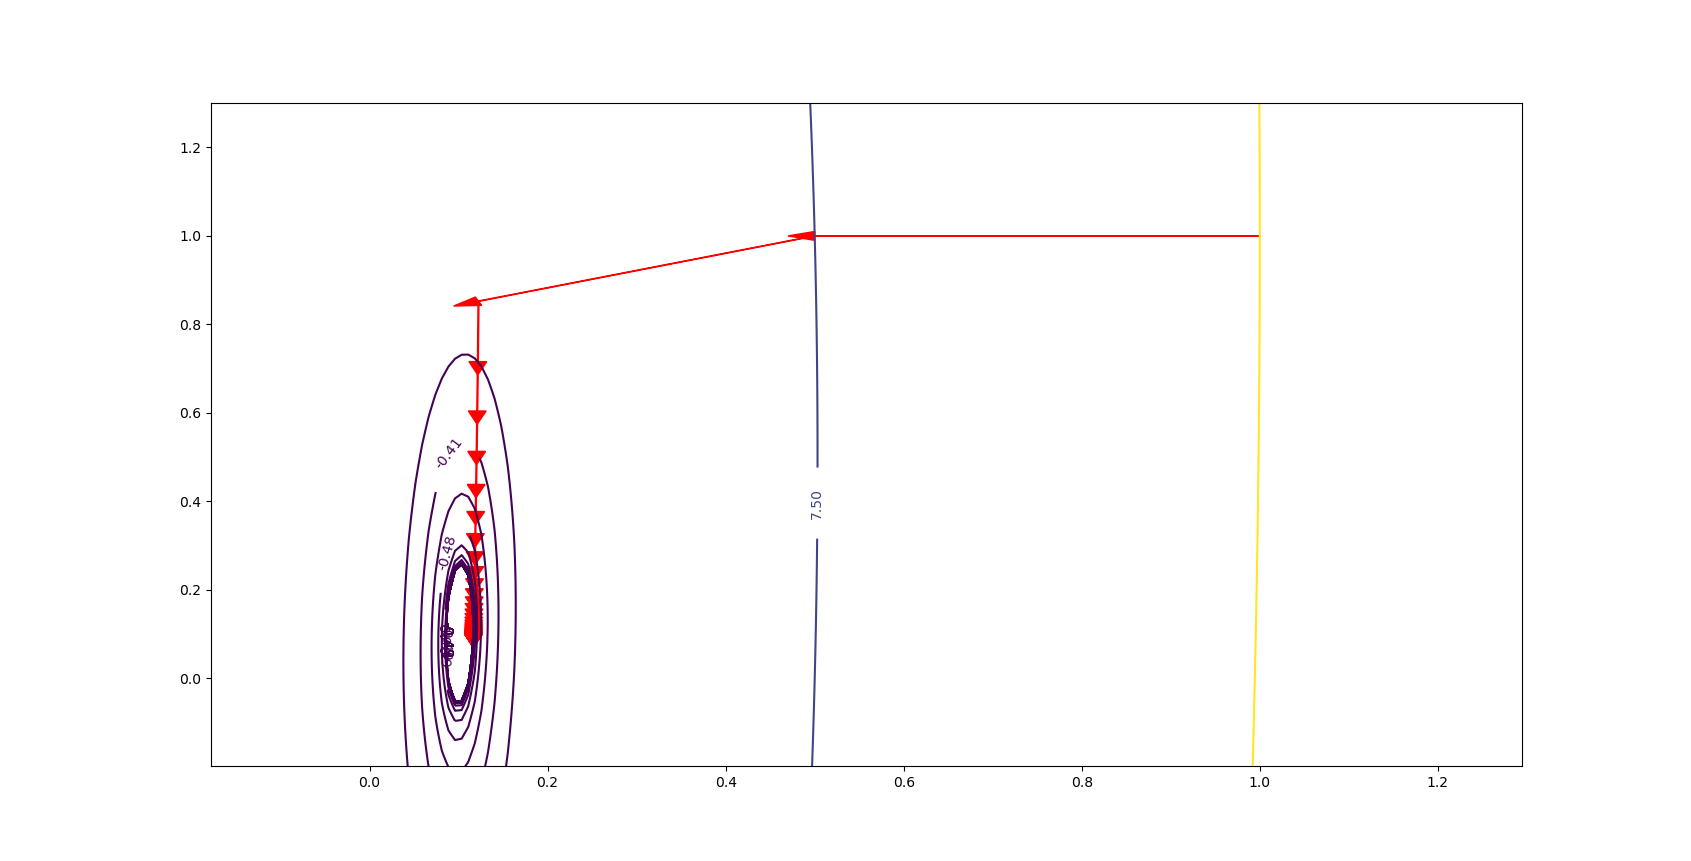
\includegraphics[H,scale=0.3]{plots/traectories/gradient_descent_1.png}
\captionof{figure}{Траектория метода на функции \(f_1\)}
\end{center}
\begin{center}
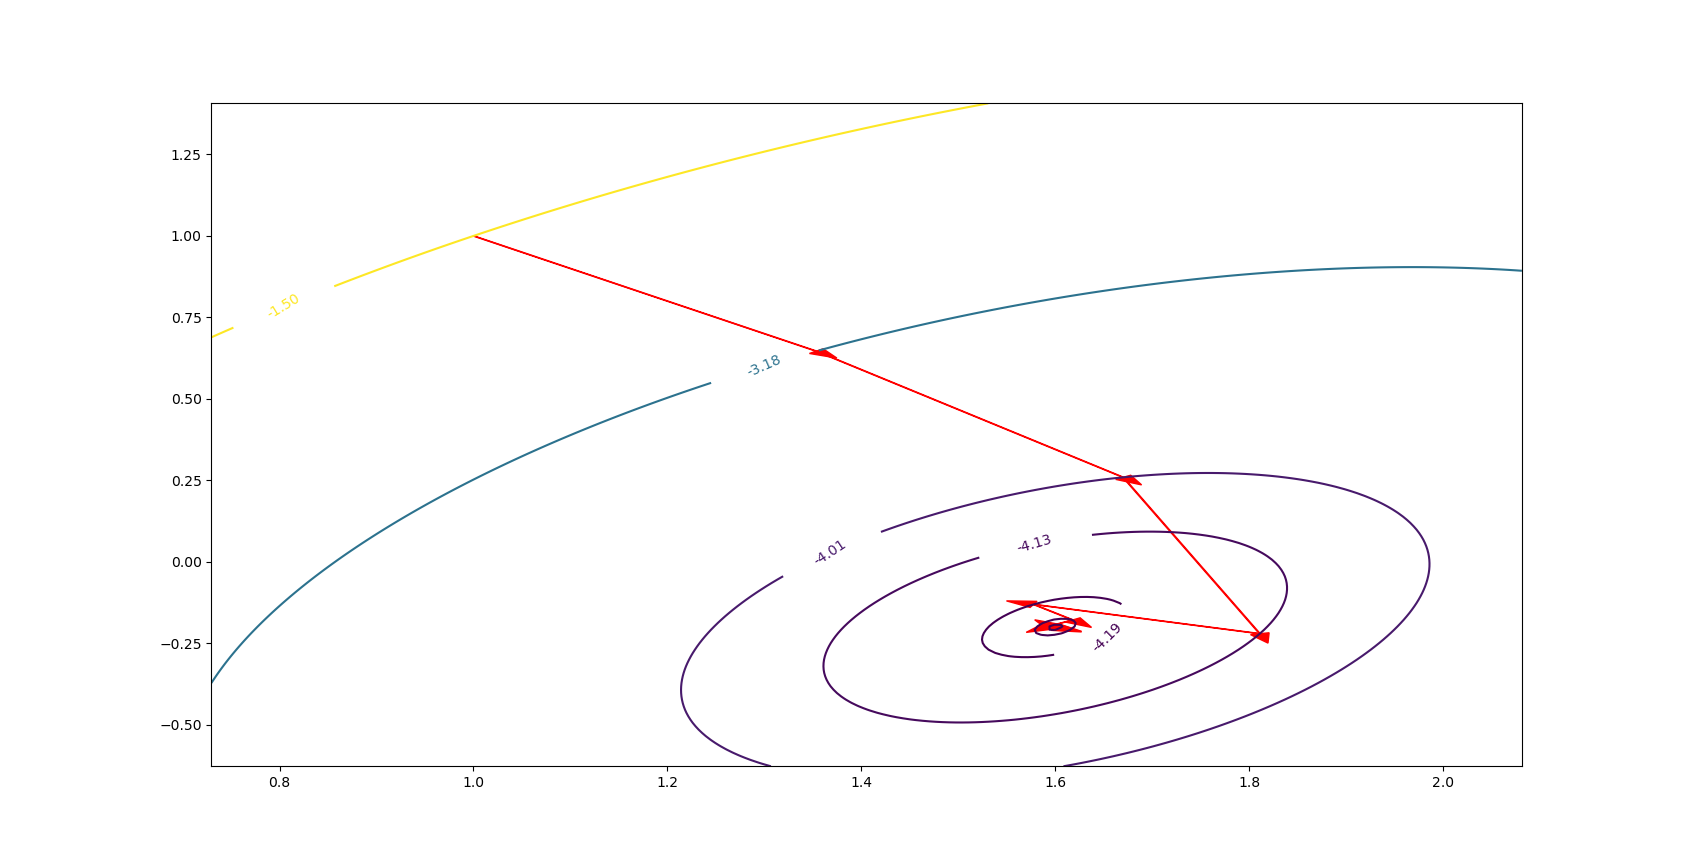
\includegraphics[H,scale=0.3]{plots/traectories/gradient_descent_2.png}
\captionof{figure}{Траектория метода на функции \(f_2\)}
\end{center}
\begin{center}
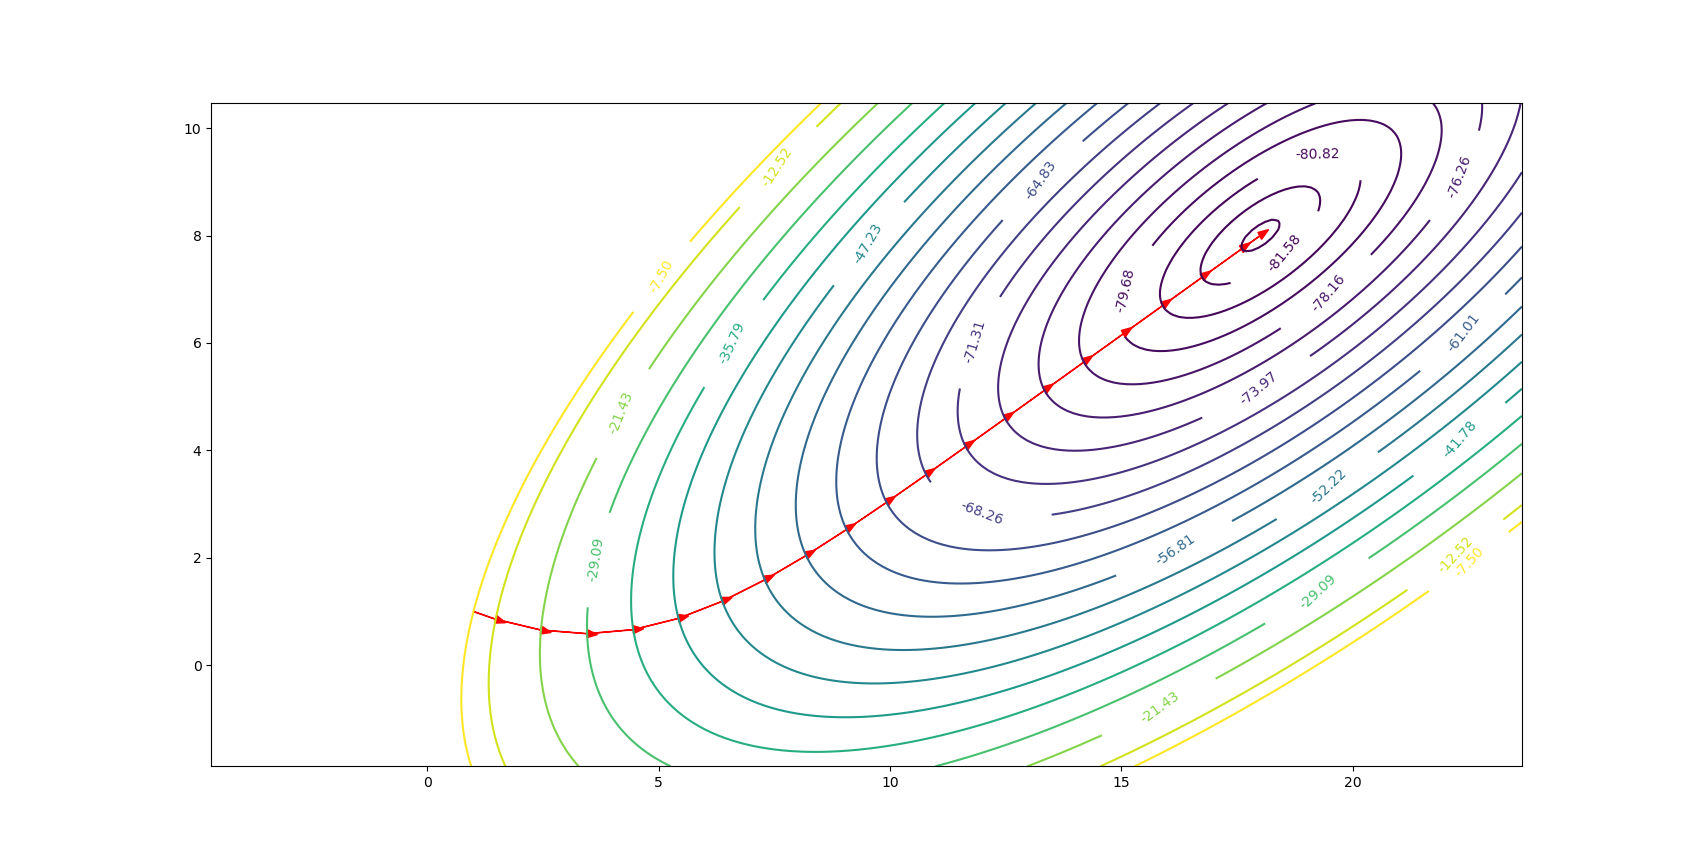
\includegraphics[H,scale=0.3]{plots/traectories/gradient_descent_3.png}
\captionof{figure}{Траектория метода на функции \(f_3\)}
\end{center}

При запуске на \(f_1\) методу потребовалось гораздо больше шагов
(\(\approx\) 800) дла нахождения минимума в отличии от функий \(f_2\)
(\(\approx\) 10 шагов) и \(f_1\) (\(\approx\) 40 шагов), так как число
обусловленности матрицы \(A\) функции \(f_1\) достаточно велико \(\mu
= 100\).
\subsubsection{Метод наискорейшего спуска}
\label{sec:org8377267}
\begin{center}
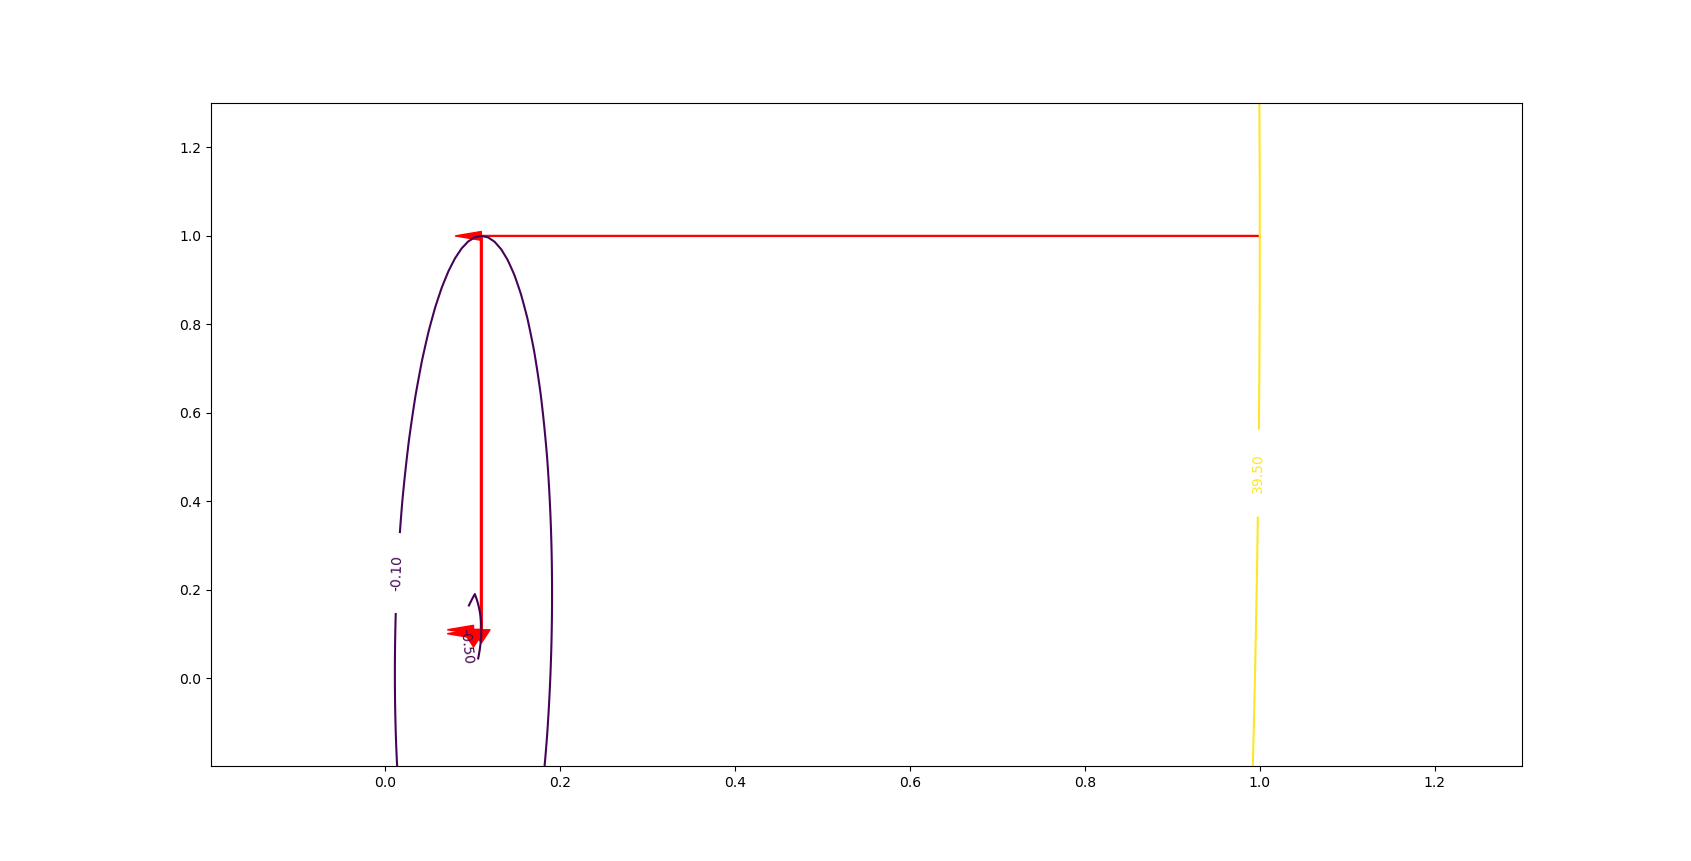
\includegraphics[H,scale=0.3]{plots/traectories/steepest_descent_1.png}
\captionof{figure}{Траектория метода на функции \(f_1\)}
\end{center}
\begin{center}
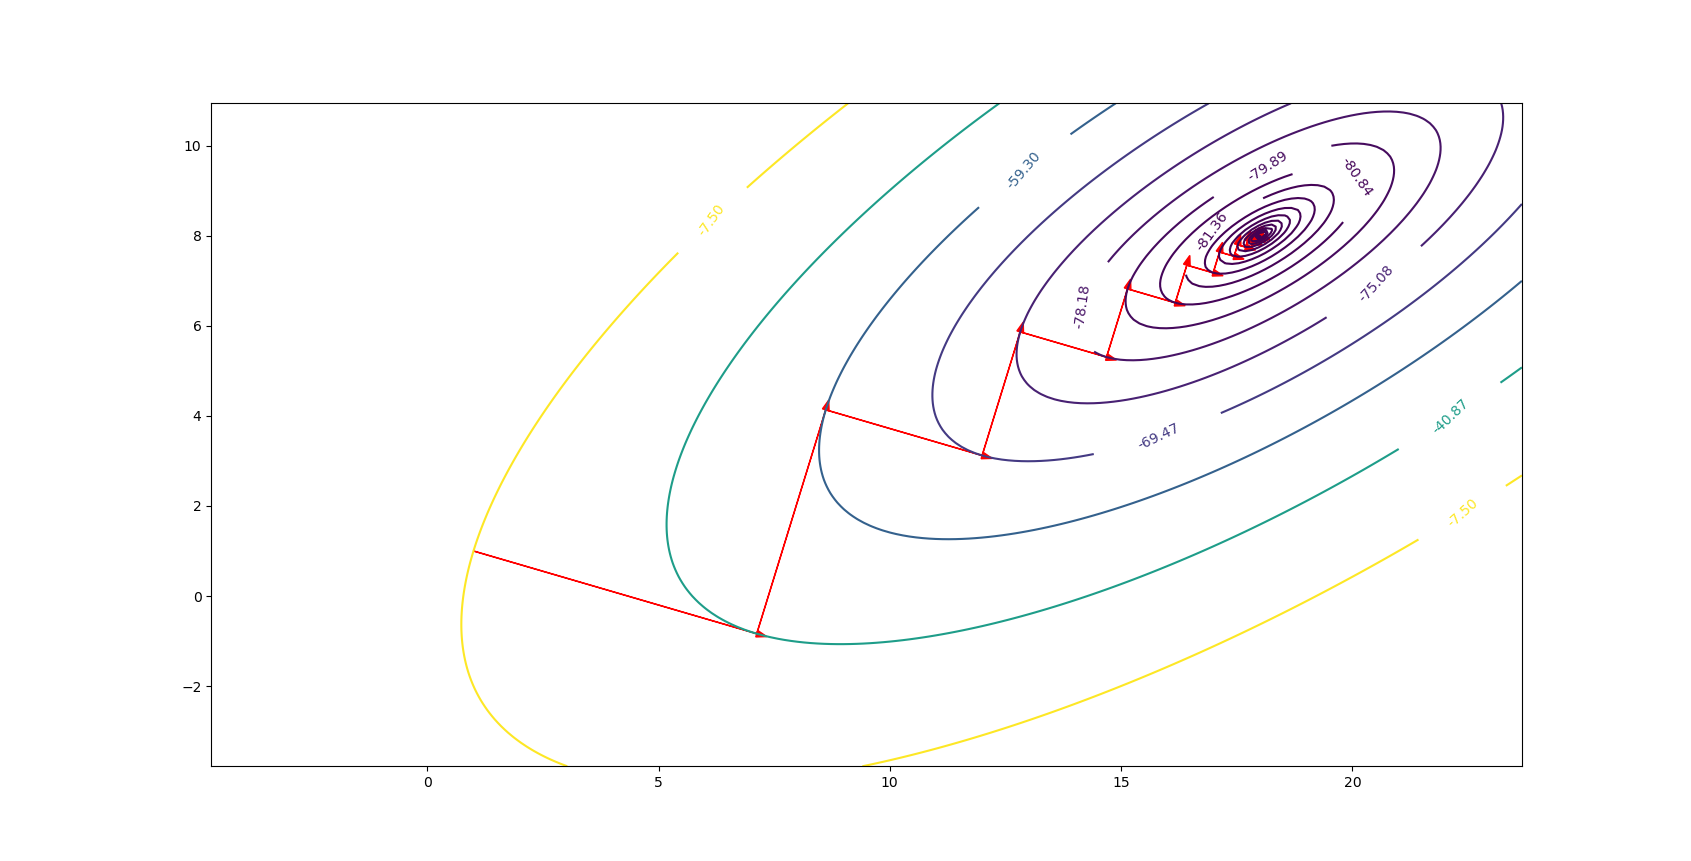
\includegraphics[H,scale=0.3]{plots/traectories/steepest_descent_3.png}
\captionof{figure}{Траектория метода на функции \(f_3\)}
\end{center}

Не смотря на высокое число обусловленности функции \(f_1\), метод
потребовалось 5 шагов для нахождение минимума. Но в то же время на
функции \(f_3\) потребовалось всего 2 шага.
\subsubsection{Метод сопряженных градиентов}
\label{sec:org7435387}
\-
\begin{center}
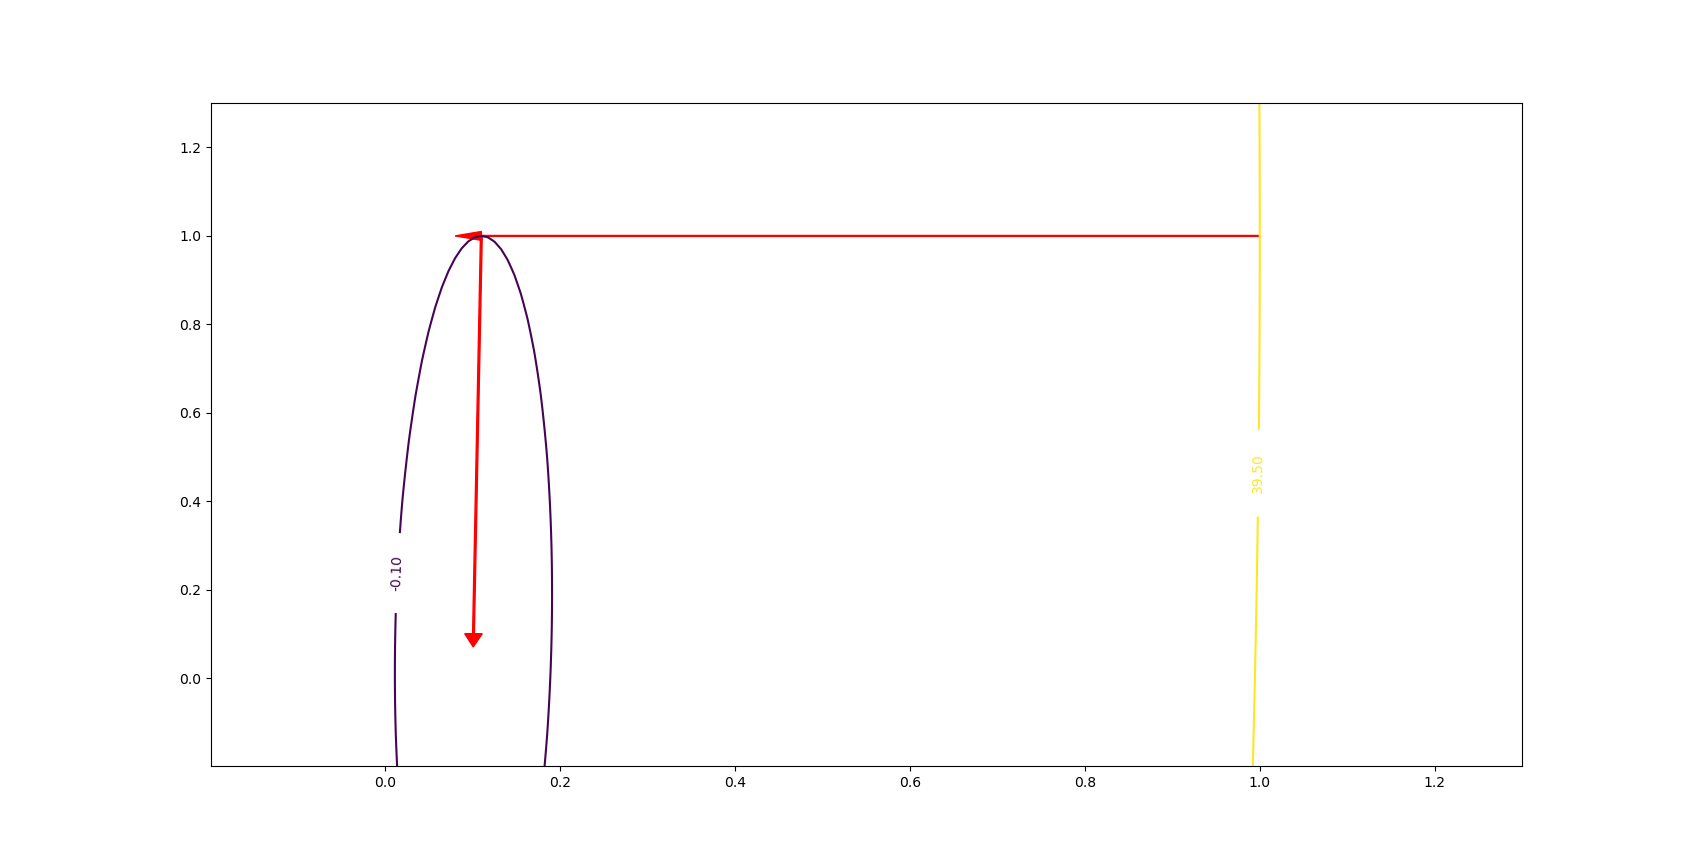
\includegraphics[H,scale=0.3]{plots/traectories/conjugate_gradient_1.png}
\captionof{figure}{Траектория метода на функции \(f_1\)}
\end{center}
\begin{center}
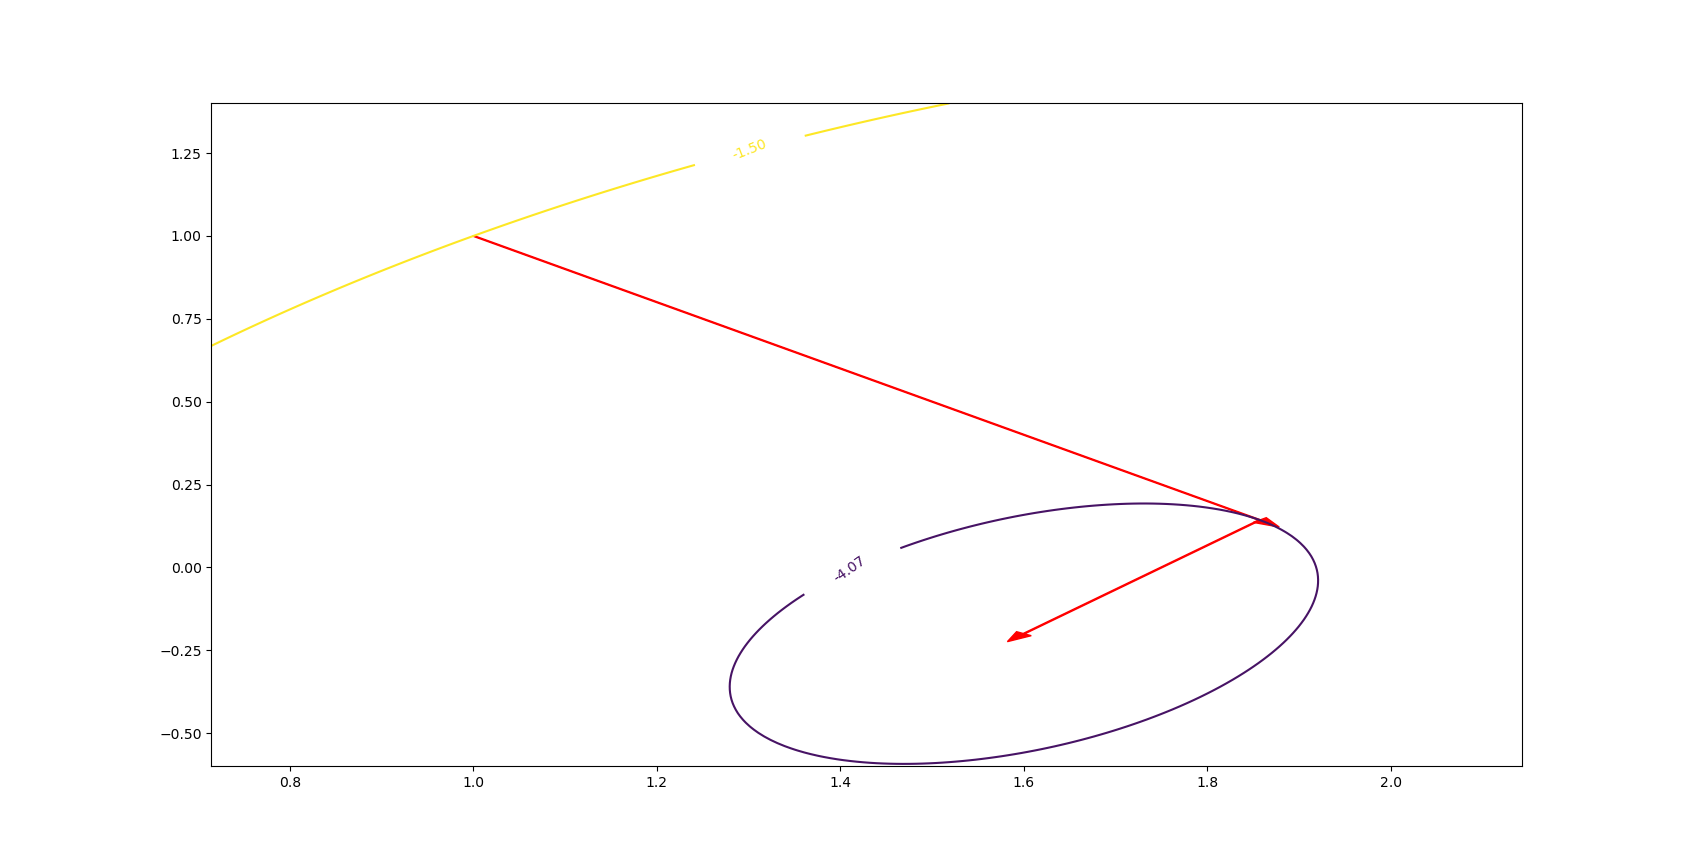
\includegraphics[H,scale=0.3]{plots/traectories/conjugate_gradient_2.png}
\captionof{figure}{Траектория метода на функции \(f_2\)}
\end{center}

В данном методе крайне редко удается добиться того, чтобы количество
итераций оказалось меньше размерности пространства
\end{document}
